% 17-17 ⑴(본책 17쪽) — 계단 모양 도로망(왼쪽 아래 2칸×1칸 블록 + 그 오른쪽 위로 2칸×2칸 블록 · 두 블록은 가운데 가로줄로 이어진다). A 왼쪽 아래 · B 오른쪽 위. 스캔 그림을 TikZ 로 다시 그림(스캔 화질).
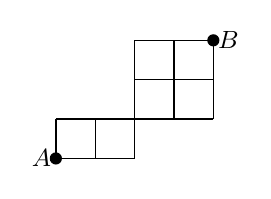
\begin{tikzpicture}[line width=0.5pt]
  % 아래 블록(가로 2칸·세로 1칸)
  \foreach \x in {0, 0.5, 1} { \draw (\x,0) -- (\x,0.5); }
  \draw (0,0) -- (1,0);
  % 두 블록을 잇는 가운데 가로줄
  \draw (0,0.5) -- (2,0.5);
  % 위 블록(가로 2칸·세로 2칸)
  \foreach \x in {1, 1.5, 2} { \draw (\x,0.5) -- (\x,1.5); }
  \foreach \y in {1, 1.5} { \draw (1,\y) -- (2,\y); }
  \fill (0,0) circle (2.2pt);
  \node[left, font=\small, inner sep=1.5pt] at (0,0) {$\pt{A}$};
  \fill (2,1.5) circle (2.2pt);
  \node[right, font=\small, inner sep=1.5pt] at (2,1.5) {$\pt{B}$};
\end{tikzpicture}
